% Generated by pipeline/paper/scripts/make_figures.py. Do not edit by hand.
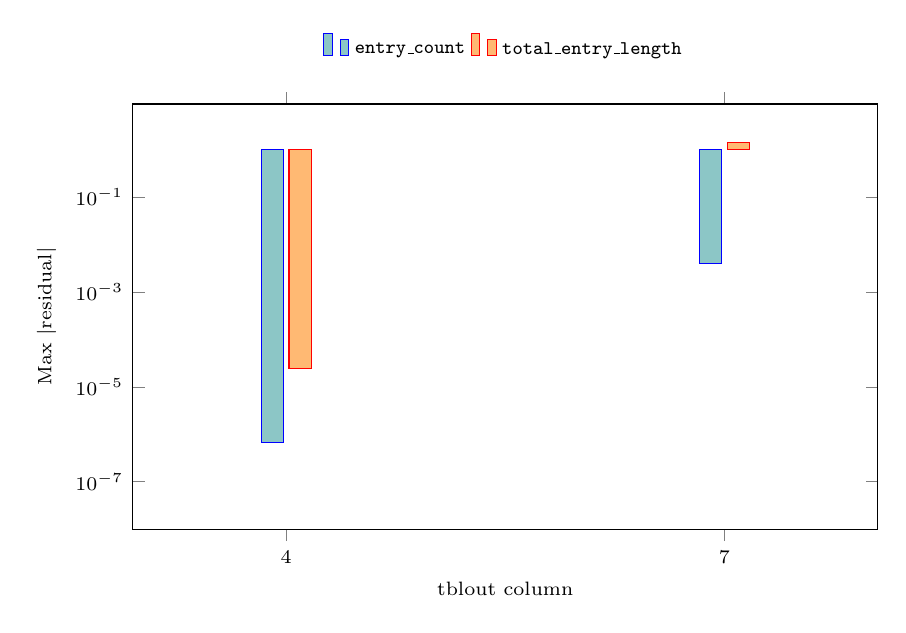
\begin{tikzpicture}
\begin{axis}[
  width=0.78\columnwidth,
  height=5.4cm,
  ybar,
  bar width=8pt,
  ymode=log,
  ymin=1e-8,
  ylabel={Max $|$residual$|$},
  symbolic x coords={4, 7},
  xtick=data,
  xlabel={tblout column},
  tick label style={font=\scriptsize},
  label style={font=\scriptsize},
  legend style={font=\scriptsize, draw=none, fill=none, at={(0.5,1.08)}, anchor=south},
  legend columns=2,
  clip=false,
  enlarge x limits=0.35,
  scale only axis,
]
% source: pipeline/results/reference_fitter_t1.json tie_break_residuals.r2p.tblout entry_count max_abs_residual
\addplot+[fill=teal!45] coordinates {(4, 6.65754174650969e-07) (7, 0.004008486175745979)};
\addlegendentry{\texttt{entry\_count}}
% source: pipeline/results/reference_fitter_t1.json tie_break_residuals.r2p.tblout total_entry_length max_abs_residual
\addplot+[fill=orange!55] coordinates {(4, 2.402989985844971e-05) (7, 1.401697018993092)};
\addlegendentry{\texttt{total\_entry\_length}}
\end{axis}
\end{tikzpicture}
